\begin{figure}[t]
\centering
    
\includegraphics[width=\linewidth]{figures/method1-refine.pdf} 
    \caption{\textbf{Architecture and Block-Based Output Representation.} LocateAnything formulates localization as generating a sequence of fixed-length, \emph{box-aligned atomic blocks}. Four functional block types—Semantic, Box, Negative, and End blocks—are defined to jointly specify predicted entities or termination states.}
    \label{fig:method1}
\end{figure}
\section{Method}

This section presents \textbf{LocateAnything}, a fast and effective framework that integrates \textbf{Parallel Box Decoding (PBD)} into VLMs for visual detection and grounding. Section~3.1 introduces the model architecture and the block-based output formulation. Section~3.2 details the joint training strategy, which aligns NTP with block-level MTP. Section~3.3 describes the on-demand inference mechanism, featuring a hybrid mode that dynamically balances decoding throughput and robustness. Finally, Section~3.4 outlines the construction of our large-scale training dataset, \textbf{LocateAnything-Data}.

\vspace{-2mm}
\subsection{Model Architecture and Formulation}

\noindent\textbf{Overview.}
As illustrated in Fig.~\ref{fig:method1}, LocateAnything builds upon a native-resolution VLM pre-trained on large-scale image-text corpora. The architecture comprises a Moon-ViT~\citep{team2025kimi} vision encoder and a Qwen2.5~\citep{qwen2.5} language decoder, bridged by a MLP projector. Given an input image \(\mathcal{I}\), the vision encoder extracts visual tokens \(Z = \text{Encoder}(\mathcal{I})\) at the native resolution, preserving the fine-grained spatial details crucial for high-precision localization. These tokens are subsequently fed into the language model, which directly converts them into a sequence of box-aligned block-level predictions.



\noindent\textbf{Block-Based Output Formulation.}
To facilitate PBD, we abandon standard NTP coordinate generation. Instead, continuous coordinates are normalized to $[0, 1000]$, discretized into tokens~\citep{jiang2025rexomni, chen2021pix2seq}, and reorganized into a sequence of blocks $\mathbf{B} = (b_1, b_2, \dots, b_N)$. Conditioned on the visual features $Z$ and a text query $\mathcal{E}$, the joint probability is formulated as $P(\mathbf{B} \mid \mathcal{Z}, \mathcal{E}) = \prod_{i=1}^{N} P(b_i \mid b_{<i}, Z, \mathcal{E})$.

Each block \(b_i\) acts as an atomic unit of constant length \(L=6\), accommodating a bounding box and two structural tokens (\eg, \texttt{<box>} and \texttt{</box>}). To guarantee uniform tensor shapes for parallel decoding, any unoccupied positions are padded with a \texttt{<null>} token. As depicted in Fig.~\ref{fig:method1}, we define four functional block types. \textit{(1) Semantic Block}: Encodes the linguistic identity. If an expression exceeds the capacity of a single block, it is partitioned across multiple consecutive blocks.
\textit{(2) Box Block}: Uses four quantized coordinates representing the bounding boxes.
\textit{(3) Negative Block}: Explicitly indicates the absence of a queried object.
\textit{(4) End Block}: Signals the termination of the generation process.


\subsection{Training Design}
Our method treats bounding box coordinates as an indivisible atomic unit, enforcing structured supervision and unlocking the capability for parallel generation. However, parallelizing the output directly in the training phase risks disrupting the model's inherent causal reasoning process. To resolve this issue, we introduce a dual-formulation training strategy that jointly optimizes two aligned representations: the NTP sequence to preserve the causal reasoning ability, and the block-wise MTP formulation for box-aligned predictions. To implement this, a single concatenated input sequence is constructed: $x_{\text{all}} = x_{\text{vis}} \oplus x_{\text{q}} \oplus x_{\text{ntp}} \oplus x_{\text{blk}}$, where \(\oplus\) denotes sequence concatenation. The terms \(x_{\text{vis}}\) and \(x_{\text{q}}\) serve as the shared context (visual and text query inputs), \(x_{\text{ntp}}\) represents the standard NTP input sequence, and \(x_{\text{blk}}\) is the block-wise MTP input sequence. Essentially, they represent the identical ground truth in two distinct formats: a \textit{token-level representation} and a \textit{block-level representation}.

Specifically, inspired by~\citep{liu2025sequential, liu2025wedlm}, \(x_{\text{blk}}\) is constructed by traversing \(x_{\text{ntp}}\) from left to right, splitting and padding the sequence according to our previously defined block rules. Within each block, we retain the first token to serve as the prediction context, while replacing all subsequent tokens with \texttt{[mask]} tokens. This structure prompts the model to simultaneously predict all masked tokens within the block in a single cohesive step. Notably, if the block size is set to 1, this MTP formulation naturally becomes equivalent to standard NTP.




\vspace{+1mm}
\begin{wrapfigure}{r}{0.52\textwidth}
    \centering
    \vspace{-5mm}
    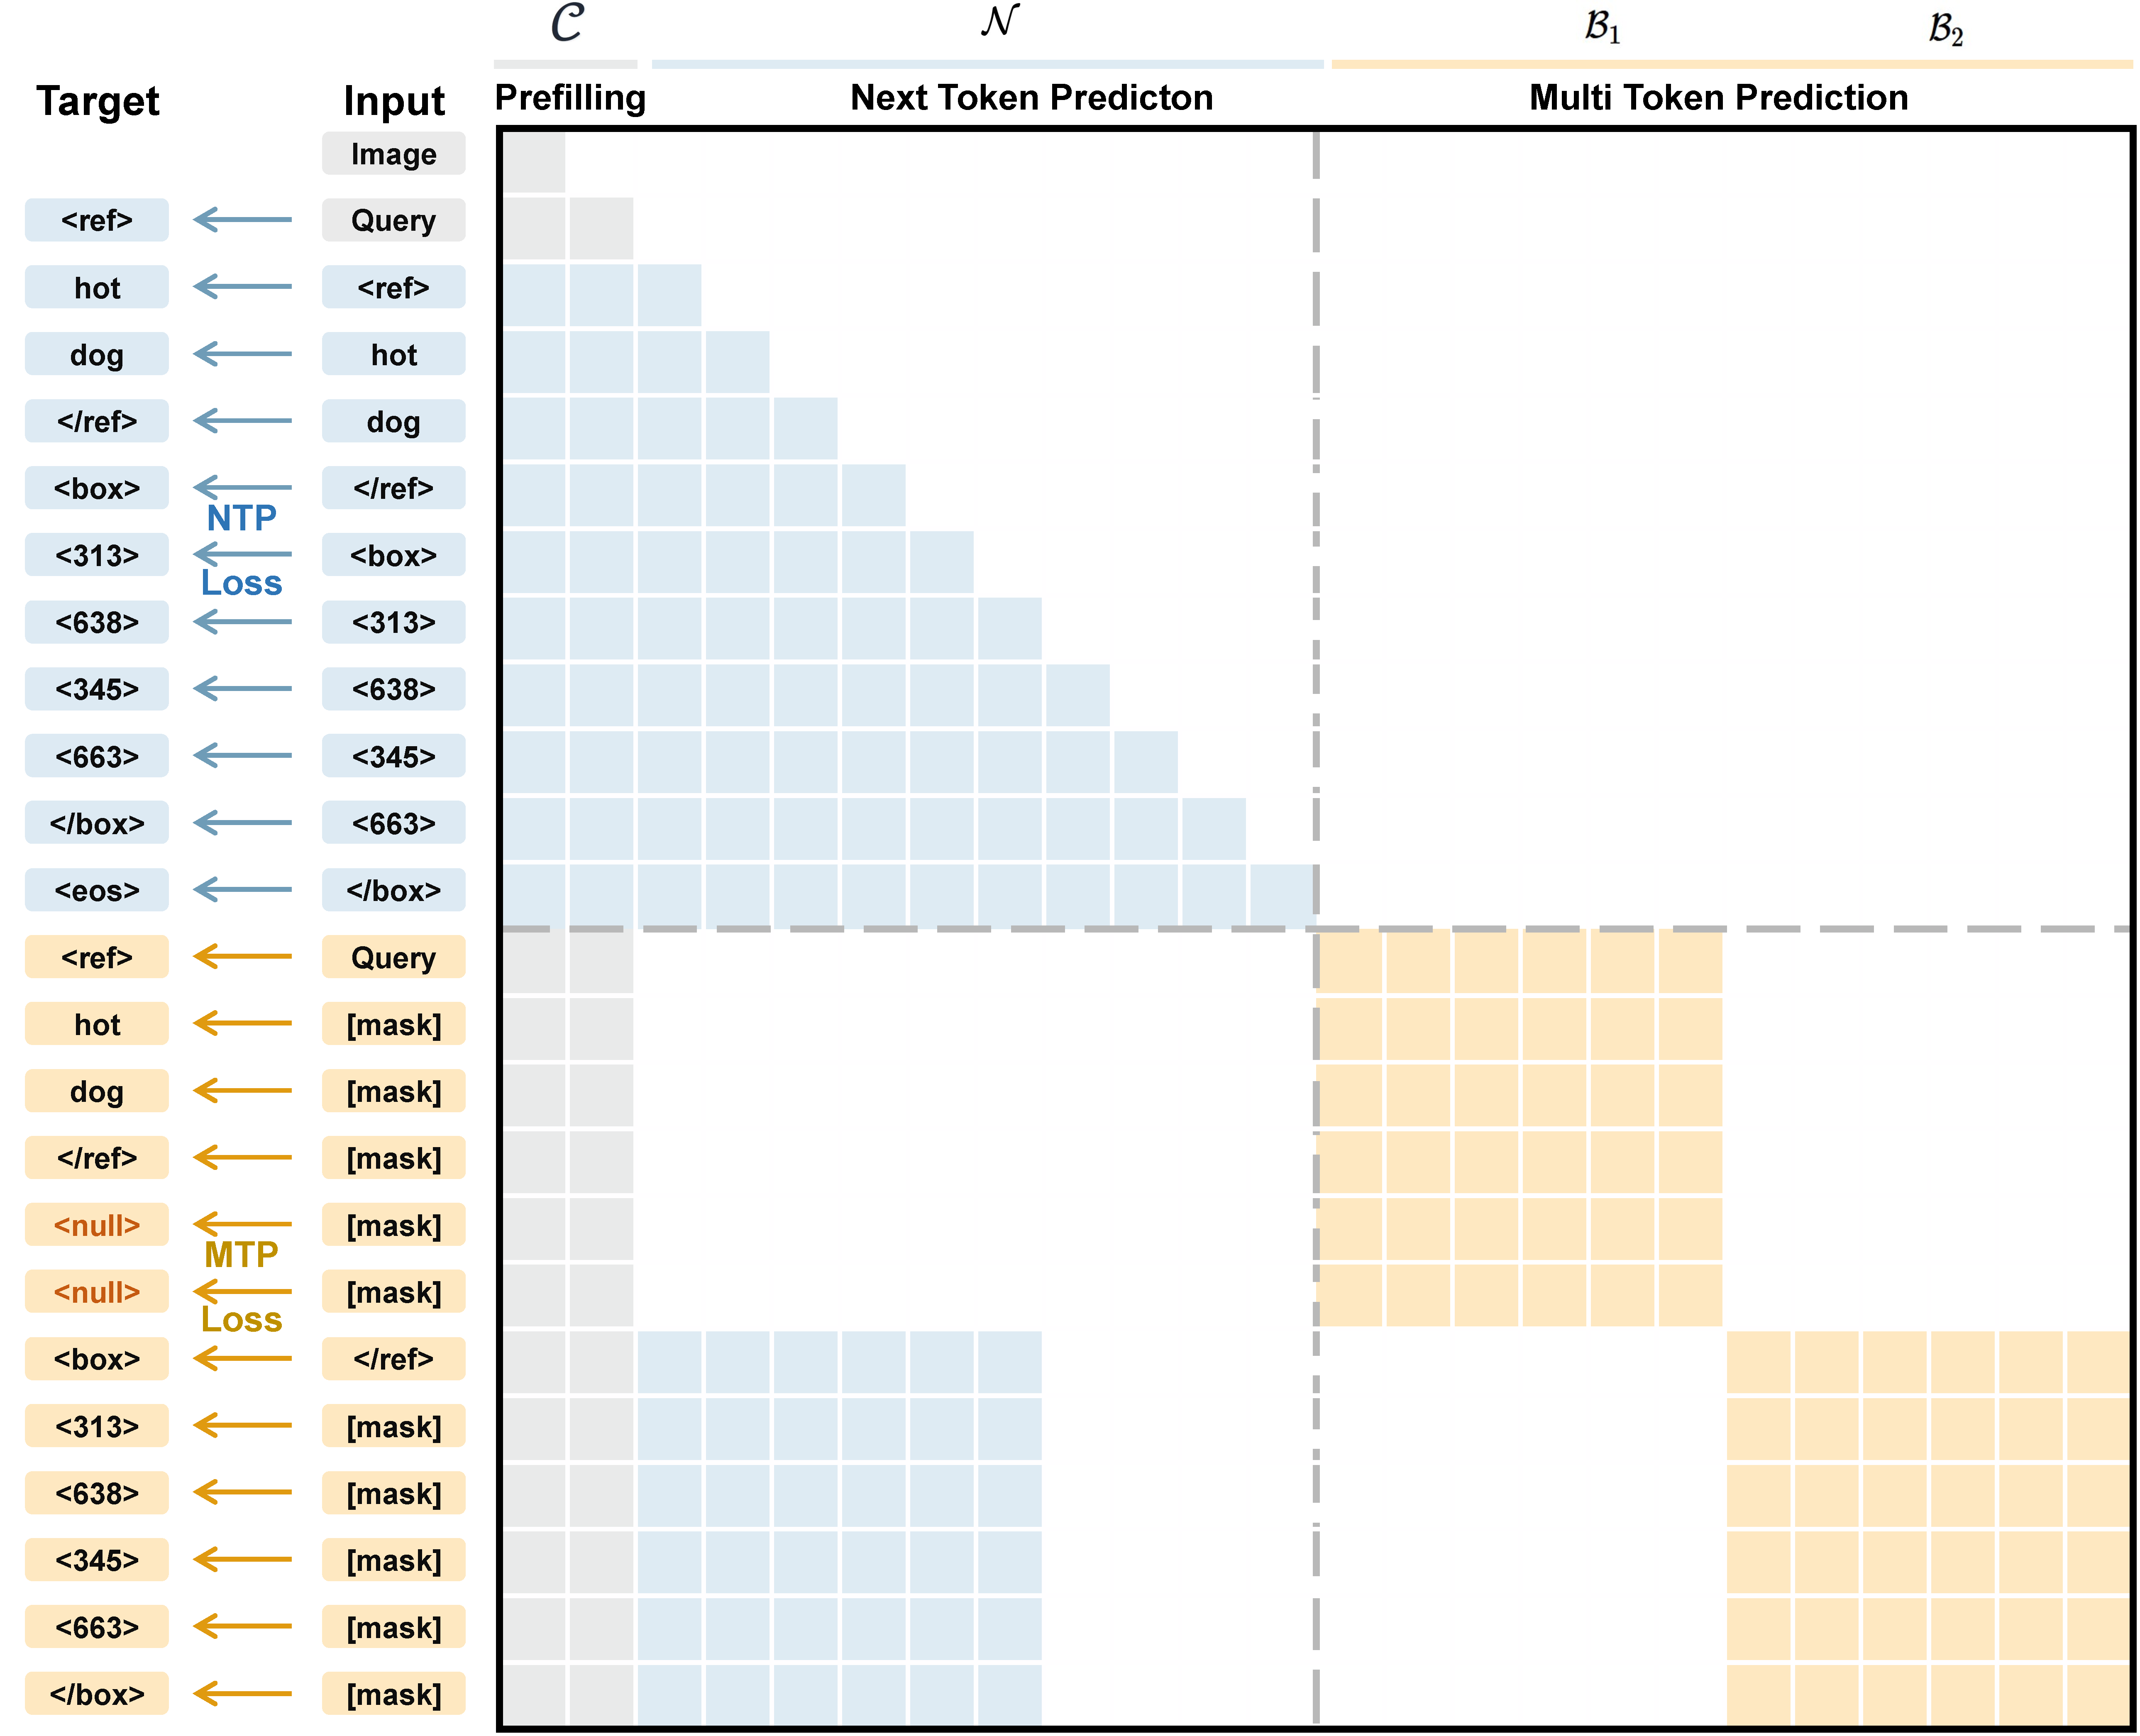
\includegraphics[width=0.5\textwidth]{figures/attn_mask.pdf}
    \vspace{-2mm}
    \caption{\textbf{Attention Mask for Joint NTP--MTP Training.} The shared context and NTP stream use causal attention, the MTP blocks follow a block-causal pattern across blocks, and tokens within the same block share bidirectional attention. The two streams are isolated to prevent leakage while jointly attending to the shared context.}
    \label{fig:attn_mask}
    \vspace{-4mm}
\end{wrapfigure}
\noindent\textbf{Attention Mask Design.} 
The core challenge of this dual-sequence formulation is how to isolate the NTP and MTP streams while allowing both to leverage the shared context. This is achieved through a specialized attention mask (as shown in Fig.~\ref{fig:attn_mask}), which dictates information flow via three distinct behaviors:
 
\noindent\textit{Causal Attention for NTP.} To preserve the original language capabilities of the VLM, the shared context (\(x_{\text{vis}}\) and \(x_{\text{q}}\)) and the NTP sequence (\(x_{\text{ntp}}\)) collectively employ a causal attention mask. Tokens within these segments can only attend to preceding tokens. Crucially, they are restricted from attending to \(x_{\text{blk}}\) to prevent data leakage. This strict causal formulation  perfectly aligns with the standard KV Cache usage during inference.

\noindent\textit{Causal Flow Across Blocks.} To align with the semi-autoregressive generation process, attention across different blocks in \(x_{\text{blk}}\) is strictly causal. Tokens in the active block can attend to the shared context and all previously committed blocks, but cannot see future blocks. This historical visibility enables the model to learn dependencies between different box predictions, effectively mitigating duplicate or missing bounding boxes.

\noindent\textit{Bidirectional Intra-Block Attention.} Following the block-causal design widely adopted in recent generative modeling~\citep{arriola2025block, nie2025large, wang2025diffusion, wu2025fast, fu2025efficient, wu2025fastv1}, tokens within the same block share bidirectional attention. This fully-connected intra-block interaction allows the model to capture complex internal relationships (\eg, geometric dependencies among a set of coordinates) and resolve all internal tokens simultaneously within a single functional unit.

\vspace{+1mm}
\noindent\textbf{Objective.} Guided by this mask, we jointly minimize the cross-entropy losses for both sequences, \ie, $\mathcal{L} = \mathcal{L}_{\mathrm{ntp}} + \mathcal{L}_{\mathrm{mtp}}$.

\begin{figure}[t]
    \centering
    
\includegraphics[width=\linewidth]{figures/method2-refine.pdf} 
    \caption{\textbf{Corrected NTP Re-decoding.} When parallel decoding encounters \textit{Format Irregularity} or \textit{Spatial Ambiguity}, the model discards the erroneous block and reverts to standard NTP to ensure robust predictions.}
    \label{fig:method2}
\end{figure}

\vspace{-2mm}
\subsection{On-Demand Inference Modes}
While our proposed PBD significantly accelerates inference, parallel decoding faces an inherent exploration-exploitation dilemma in highly complex scenes, as shown in Fig.~\ref{fig:method2}. The first is \textit{Format Irregularity}, which occurs in complex scenes containing multiple instances across categories. During parallel decoding, the model may struggle at category boundaries, hesitating between continuing to predict for the current class or transitioning to a new class. This uncertainty manifests as malformed syntax within a single predicted block, erroneously mixing structural and coordinate tokens (\eg, \texttt{<box><211></ref><911><887></box>}). The second is \textit{Spatial Ambiguity}, which arises when objects are densely arranged in regular grids, such as rows or columns. The MTP approach can blur spatial boundaries and output an intermediate coordinate situated between two objects, consequently producing low IoU predictions.

Both failure patterns can be effectively resolved using an NTP fallback mechanism. The NTP prediction can achieve higher precision when handling complex category transitions and dense spatial layouts. Therefore, during MTP inference, we continuously validate the syntactic integrity and monitor spatial confidence. Specifically, an ambiguity trigger is activated if two conditions are met simultaneously: (1) the top-1 coordinate token's probability is below 0.7, and (2) the max-min difference among the top-5 coordinate tokens exceeds 80 within the [0, 1000] normalized space. Upon detection of a format violation or high spatial ambiguity, the compromised block is discarded, and the generation reverts to the last verified prefix. NTP is then employed to autoregressively generate the tokens for the specific problematic block. Once the block is completed, the model seamlessly switches back to MTP for subsequent predictions.

Based on the above discussion, we propose three on-demand inference modes to balance throughput and spatial robustness.
\textit{(1) Slow Mode}, which generates the output token-by-token using standard NTP.
\textit{(2) Fast Mode}, which leverages MTP to predict box-aligned blocks. For each block, \texttt{<null>} padding tokens are discarded, and the remaining tokens are appended to the output; the committed tokens are stored in the key-value cache and serve as causal context for subsequent prediction steps.
\textit{(3) Hybrid Mode}, which employs MTP by default but seamlessly switches to NTP when parallel outputs become unreliable.

\vspace{+1mm}
\noindent\textbf{Inference-Time Attention Mask.}
During inference, the attention mask for each MTP decoding step mirrors the training-time block-causal pattern illustrated in Fig.~\ref{fig:attn_mask}. All previously committed tokens in the KV cache follow standard causal attention, while the $n_{\text{future}}$ tokens in the current MTP block attend to each other bidirectionally, enabling parallel token prediction. Meanwhile, the current block can attend to all preceding blocks but is prevented from accessing subsequent ones. After each MTP step, the KV cache is truncated to retain only committed tokens, evicting mask tokens and the duplicated anchor to ensure the cache stays consistent with the causal prefix seen during training.

\begin{figure*}[t]
    \centering
    
\includegraphics[width=\textwidth]{figures/data.pdf}
    \caption{Overview of the \textbf{LocateAnything-Data} dataset. The pie charts illustrate the task distribution across natural language queries, bounding boxes, and unique images. The bottom panel provides a detailed breakdown specifically for the language queries, showing the absolute count and percentage for each task category.}
    \label{fig:dataset_stats}
\end{figure*}

\subsection{LocateAnything-Data}
\label{sec:dataset}

To train a highly capable model for general-purpose visual detection and grounding, we curate \textbf{LocateAnything-Data}, a large-scale, multi-domain dataset. The dataset construction details can be found in the \textbf{supplementary}. 

As illustrated in Fig.~\ref{fig:dataset_stats}, the dataset contains 12M unique images and 138M natural language queries. Furthermore, the dataset includes 785M annotated bounding boxes, providing massive and dense supervisory signals to guide the spatial learning of the LocateAnything model. The training corpus is categorized into six distinct tasks. (1) \textbf{General object detection} constitutes the foundation, representing 66.9\% of the queries and providing the essential bounding box supervision (83.1\%) to help the model achieve precise and dense coordinate alignments. (2) \textbf{Grounding user interface} elements (16.5\% of queries) enable the model to support embodied agents and graphical user interface navigation tasks. (3) \textbf{Natural language referring} comprehension (7.3\% of queries) enables the model to link complex linguistic intents to specific spatial regions. (4) \textbf{Text localization} (3.6\% of queries) ensures that the model can perceive and tightly ground textual information within images. (5) \textbf{Document and scene layout grounding} (3.5\% of queries) enriches the structural reasoning capabilities of the model. (6) \textbf{Point-based localization} tasks (2.2\% of queries) further refine the spatial precision of the model for fine-grained predictions.
